\chapter {Fase II: Diseño}
\label{cap:Fase II.Diseño}
En el diseño de sistemas informáticos se suelen usar las arquitecturas multinivel o programación por capas, en la que a cada nivel se le confía una misión simple. Para el desarrollo de nuestra aplicación nos hemos marcado como objetivo el desacomplamiento de las diferentes partes que componen el sistema: capa de presentación, capa de datos y capa de lógica de negocios. En este sentido, comenzamos el proyecto diseñando la interfaz de usuario, continuamos modelando la parte lógica y terminamos añadiendo persistencia de datos.

\section{Presentación. Prototipo de la GUI}

Una vez identificados los requisitos de la aplicación, nos hemos centrado en la creación de bocetos de baja fidelidad de la aplicación. En esta parte, nos hemos preocupado por el diseño de ventanas y posicionamiento de los controles, así como en el diseño de formularios y listados de información. Para ello, nos hemos basado en los conceptos teóricos vistos en la asignatura\textbf{\emph{ Interacción Persona-Ordenador}}, como empleo de metáforas, selección adecuada de colores y, sobre todo los aspectos relacionados con principios de usabilidad (flexibilidad, adaptabilidad, consistencia, etc.) y Leyes de Gestalt.

En este sentido, hemos utilizado la aplicación Balsamiq Mockups para realizar un prototipado horizontal que incluye la interfaz de todas las características del sistema, pero sin funcionalidad subyacente. En las capturas que se adjuntan a continuación, se incluyen los bocetos de baja fidelidad que creamos en una primera fase del proyecto, y que consecuentemente, pueden haber sufrido modificaciones con respecto al aspecto final de la aplicación. 


\subsubsection{Ventana de Inicio}
\begin{wrapfigure}{l}{0.3\linewidth}
    \centering
    \includegraphics[width=1\linewidth]{GSI-1}
    \caption{{Ventana de Inicio}}
    \label{fig:GES1}
\end{wrapfigure}
Para que la aplicación permita monitorizar la evolución del RCV y pueda utilizarse como una herramienta motivacional para el paciente, hemos considerado obligatoria la necesidad de diseñar una ventana de \emph{login}, como paso previo a la utilización de las funciones de la aplicación. 

De esta forma, se podrá registrar cada uno de los cálculos realizados por el usuario y mostrar un gráfico con la evolución del RCV. Además, al disponer de cierta información personal sobre el usuario, no será necesario que introduzca algunos datos necesarios para realizar el cálculo.

Una vez autenticado, la navegación por la aplicación se basará en una barra de navegación situada en la parte inferior de la pantalla y que ofrecerá la posibilidad de desplazarse por tres ventanas: estado, nuevo cálculo y perfil. Una de las razones que nos llevan a tomar esta decisión de diseño, es que la barra de navegación inferior se encuentra dentro de la ‘thumb zone’, que es el área que puede alcanzar el usuario cuando sujeta el móvil con una sola mano utilizando el pulgar para navegar. De esta forma, permite navegar rápidamente entre las principales vistas del menú de la app. 

\subsubsection{Ventana de Estado}

\begin{wrapfigure}{r}{0.3\linewidth}
	\centering
	\subfigure[Ventana de Estado]{
			\includegraphics[width=0.3\textwidth]{GSI-2}
			\label{fig:graficoSE}
		}
		\subfigure[Ventana de Perfil]{
			\includegraphics[width=0.3\textwidth]{GSI-3}
			\label{fig:tablaSE}
		}
		\caption[Ventana de Perfil y Estado]{Ventana de Perfil}
	
	\label{fig:defPerfil}
\end{wrapfigure}
La primera de las opciones seleccionables en el menú de navegación será la denominada Estado. En ella, se mostrará información relativa al último cálculo de RCV realizado por el usuario que ha iniciado sesión. Para ello, en la parte superior de la pantalla se mostrará un gráfico circular con el porcentaje de riesgo calculado y la fecha del mismo. Horizontalmente alineado con esta información aparecerá una etiqueta en la que se clasifique ese último cálculo en riesgo alto, moderado o bajo, de acuerdo con la tabla ~\ref{fig:tablaFir2}.

Por otro lado, se incluirá un listado dinámico con información sobre los factores de riesgo utilizados para realizar el cálculo. En este sentido, aparecerá información sobre la abstención o no de tabaco por parte del usuario, actividad física, tensión arterial, colesterol y si el usuario está en su peso ideal de acuerdo basándose en un cálculo del índice de masa corporal (IMC).


\subsubsection{Ventana de Perfil}
Lo más destacable de la ventana que se mostrará al seleccionar la opción del menú Perfil, es que se incluirá un gráfico que permita monitorizar la evolución del RCV. En el eje de las ordenadas se representará el porcentaje de riesgo cardiovascular, mientras que en el eje X se dimensionará la fecha en la que se realizó el cálculo.

Además del gráfico, en esta ventana se mostrarán los datos personales del usuario: nombre, apellidos, fecha de nacimiento y fecha de último acceso a la aplicación. 

\subsubsection{Ventana de Cálculo del RCV}
Seleccionando la opción Cálculo del menú de navegación de la aplicación el usuario podrá realizar una estimación del riesgo cardiovascular. Como sabemos, para poder aplicar el algoritmo de Framimgham, es necesario haber obtenido previamente una serie de información concreta relevante al usuario. Estamos haciendo referencia a los factores de riesgos de los que hablamos en la sección de Análisis (\ref{cap:Fase I. Análisis}). 

Esta ventana mostrará un formulario en el que se solicitará al usuario que introduzca su peso, altura, tensión arterial, si es o no fumador, colesterol (HDL y total), nivel de actividad física (un día por semana, dos días por semana, nada o una vez al mes) y enfermedades que puedan afectar al cálculo del RCV como la diabetes, hipertensión arterial o hipertrofia del ventrículo izquierdo.

\begin{figure}[htb]
	\centering
	\subfigure[]{
		\includegraphics[width=0.3\textwidth]{GSI-4} 
		\label{fig:raCalculo1}
	}

		\subfigure[]{
			\includegraphics[width=0.3\textwidth]{GSI-9}
			\label{fig:raCalculo6}
		}
		\subfigure[]{
			\includegraphics[width=0.3\textwidth]{GSI-10}
			\label{fig:raCalculo7}
		}
	\caption{Ventana Cálculo del RCV}
	\label{fig:cirugiaRA}
\end{figure}


\section{Dominio}
Dentro de la lógica de negocio, los usuarios se representan como objetos de la clase \emph{\textbf{Usuario}} con una serie de propiedades para realizar la autenticación: correo electrónico y pass. Además, para permitir el control de la evolución del RCV, cada objeto usuario almacena un \emph{array} con el historial de cálculos asociados a ese usuario. Un cálculo está definido mediante un objeto de la clase \textbf{\emph{CalculoRCV}}, la cual contiene atributos y métodos necesarios para encapsular una estimación de riesgo cardiovascular. Esta es la razón de la unión mediante una relación de asociación entre la clase Usuario y CalculoRCV.

Al mismo tiempo, la clase CalculoRCV contiene como atributo un objeto de la clase \textbf{\emph{FactoresRCV}}, la cual se utiliza para encapsular los factores de riesgo que se mostrarán en el listado dinámico que explicamos en la parte de presentación.


Por otro lado, hemos definido una \emph{interface} \textbf{\emph{ConstantesFactores}} para definir todas las propiedades constantes utilizadas para la estimación de RCV y recomendaciones de actuación. En este sentido, en esta interfaz definidos como constantes los valores límites para el colesterol, tensión y resultados del cálculo. Esta interfaz es implementada por las clases \emph{FactoresRCV} y \emph{CalculoRCV}.

Finalmente la clase \emph{\textbf{FraminghamRiskScore}} contiene los métodos necesarios para calcular el porcentaje de riesgo cardiovascular según las tablas de Framimgham. Adjuntamos el código Java en el anexo \ref{cap:AnexoA}.


\begin{figure}[H]
	\centering
	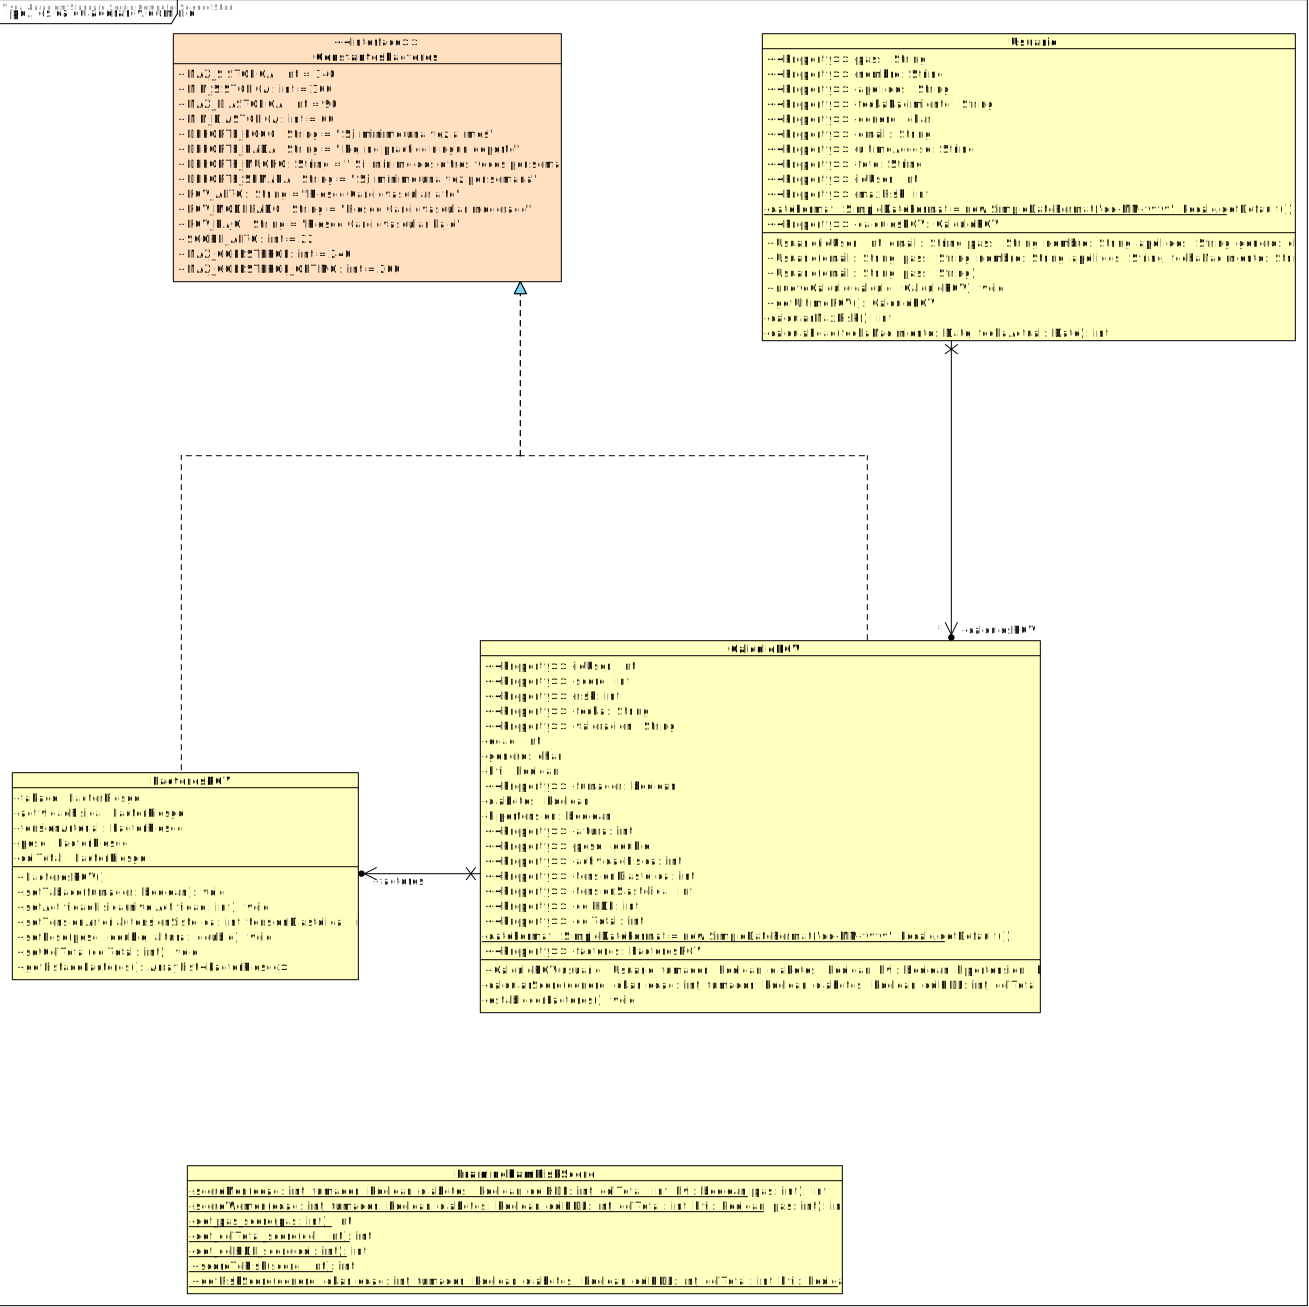
\includegraphics[width=\textwidth]{diagramClases} 
	\caption[Diagrama de clases]{Diagrama de clases UML de la capa de dominio
	}
	\label{fig:diagramaClases}
\end{figure}

\pagebreak



\section {Persistencia. BBDD Local}
Dentro de los distintos sistemas de bases de datos tanto privativos como libres/open source (Oracle, SQLServer, MySQL, etc) existe uno que se adapta perfectamente a las aplicaciones móviles:\textbf{ SQLite.} El principal motivo es que SQLite no requiere más que un simple fichero para almacenar los datos, ya que la lógica de funcionamiento debe ser implementada por la plataforma que desee interactuar con los datos.

\noindent Una vez decida la plataforma de BBDD que ibamos a utilizar en nuestra aplicación, era el momento de diseñar la estructura de la misma. Simplemente necesitamos modelar dos tablas: una para almacenar la información de los usuarios registrados en el sistema, indexada por un identificador único de usuario; y otra tabla en la que se almacenen todos los cálculos realizados en el sistema. Las dos tablas están relacionadas a través del identificador de usuario. 

Las siguientes imágenes muestran el código SQL de creación de las dos tablas que forman la base de datos de nuestra aplicación. 

\begin{figure}[htb]
	\centering
		\subfigure[Tabla Usuario]{
			\includegraphics{userTabla}
			\label{fig:tablaUsuario}
		}
	\subfigure[Tabla CalculosRCV]{
		\includegraphics{calculoTabla}
		\label{fig:tablasCalculos}
	}

	\caption{Código creación de tablas SQLite}
	\label{fig:sqlite}
\end{figure}

\subsubsection{Implementación en Android}
El procedimiento recomendado para crear una nueva base de datos SQLite en Android, se resume de forma esquemática:
\begin{itemize}
\item Crear una \textbf{clase} que extienda de \textbf{\emph{SQLiteOpenHelper}}. En nuestro caso, la hemos llamado \emph{DB\_Helper}.

\item Sobreescribir en ella el método \textbf{\emph{onCreate()}}, donde se ejecutará un comando SQLite para crear las tablas de la base de datos.

\item También es necesario sobrescribir el método \textbf{\emph{onUpgrade}}, el cual se ejecutará cada vez que cambiamos la versión de la base de datos, y se usará para migrar los datos de la base de datos anterior a la nueva versión. 
\end{itemize}

El siguiente listado de código muestra los métodos \emph{onCreate} y \emph{onUpgrade} de la clase DB\_Helper, utilizada como conector en nuestra aplicación. 

\lstinputlisting[style=Java-color,caption={Clase DB\_Helper.java},label=lst:codCfile]{./code/DB_Helper2.java}




